\documentclass[german,a4]{scrartcl}


\usepackage{tikz}
\usetikzlibrary{mindmap}
\usetikzlibrary{arrows,shapes,snakes,automata,backgrounds,petri,decorations.markings,calc,decorations.pathmorphing,patterns,fadings}

\pgfdeclaredecoration{penciline}{initial}{
    \state{initial}[width=+\pgfdecoratedinputsegmentremainingdistance,auto corner on length=1mm,]{
        \pgfpathcurveto%
        {% From
            \pgfqpoint{\pgfdecoratedinputsegmentremainingdistance}
                            {\pgfdecorationsegmentamplitude}
        }
        {%  Control 1
        \pgfmathrand
        \pgfpointadd{\pgfqpoint{\pgfdecoratedinputsegmentremainingdistance}{0pt}}
                        {\pgfqpoint{-\pgfdecorationsegmentaspect\pgfdecoratedinputsegmentremainingdistance}%
                                        {\pgfmathresult\pgfdecorationsegmentamplitude}
                        }
        }
        {%TO 
        \pgfpointadd{\pgfpointdecoratedinputsegmentlast}{\pgfpoint{1pt}{1pt}}
        }
    }
    \state{final}{}
}

\usepackage{color}

\usepackage{listings}

\lstset{language=XML,
%  otherkeywords={stream,container,process,service},
  basewidth={0.5em,0.45em},
  fontadjust=false,
  basicstyle=\footnotesize\ttfamily,
  keywordstyle=\color{blue},          % keyword style
  commentstyle=\ttfamily\color{black!60},       % comment style
  showstringspaces=false,
  stringstyle=\color{darkGreen},
  keywordstyle=[2]{\color{blue}},
  morekeywords=[3]{org.jwall.example.Identity}
}

\lstdefinelanguage{JavaScript}{
  keywords={typeof, new, true, false, catch, function, return, null, catch, switch, var, if, in, while, do, else, case, break},
  keywordstyle=\color{blue}\bfseries,
  ndkeywords={class, export, boolean, throw, implements, import, this},
  ndkeywordstyle=\color{darkgray}\bfseries,
  identifierstyle=\color{black},
  sensitive=false,
  comment=[l]{//},
  morecomment=[s]{/*}{*/},
  commentstyle=\color{purple}\ttfamily,
  stringstyle=\color{red}\ttfamily,
  morestring=[b]',
  morestring=[b]"
}

\lstdefinelanguage{Java}{
  keywordstyle=[2]{\color{javaKeyword}},
  keywordstyle=[3]{\color{javaType}},
  keywordstyle=[4]{\color{blue}},
  stringstyle=\color{javaString}\ttfamily,
  morekeywords=[2]{public,class,final,protected,implements,return,package,import},
  morekeywords=[3]{Data,org.jwall.example,Identity}
}


\definecolor{lila}{rgb}{0.5019,0.0000,0.5019}

\definecolor{gruen}{rgb}{0.7019,0.7725,0.4470}
\definecolor{gruenRand}{rgb}{0.4,0.4509,0.2117}

\definecolor{hellgruen}{rgb}{0.8745,0.9215,0.7725}
\definecolor{hellgruenRand}{rgb}{0.6823,0.7137,0.5843}

\definecolor{hellblau}{rgb}{0.8196,0.9137,1.0}
\definecolor{hellblauRand}{rgb}{0.6275,0.6941,0.7647}

\definecolor{blauRand}{rgb}{0.2078,0.3019,0.4196}
\definecolor{blau}{rgb}{0.4,0.5686,0.7686}

\definecolor{lila}{RGB}{204,204,255}
\definecolor{lilaRand}{RGB}{146,137,188}

\definecolor{rapidi}{RGB}{240,176,0}
\definecolor{rapidiText}{RGB}{102,51,0}
\definecolor{darkGreen}{RGB}{67,101,0}


\definecolor{orange}{rgb}{1.0,0.8509803921568627,0.6549019607843137}
\definecolor{orangeRand}{rgb}{0.9725,0.6941,0.5017}

\definecolor{dunkelOrange}{RGB}{215,111,1}

\definecolor{xmlString}{RGB}{67,101,0}

\definecolor{javaKeyword}{rgb}{0.4980,0.0,0.3333}
\definecolor{javaString}{rgb}{0.16470588235294117,0.0,1.0}
\definecolor{javaType}{rgb}{0.0050980392156,0.39215686274509803,0.0}


\definecolor{gruen1}{RGB}{105,193,16}
\definecolor{gruen2}{RGB}{197,232,162}
\definecolor{gruen3}{RGB}{138,206,67}
\definecolor{chaptergruen}{RGB}{88,152,10}

\definecolor{pinkRand}{RGB}{255,153,153}
%!TEX root = ./stream-processing-survey.tex
% \DeclareMathOperator{\data}{Data}

\newcommand{\chapterQuoteText}{}
\newcommand{\chapterQuoteAuthor}{}

\newcommand{\theChapterQuote}{}

\renewcommand{\theChapterQuote}{
{\normalsize\textnormal{
\hfill\begin{minipage}{0.9\textwidth}
\begin{flushright}
	{\em \chapterQuoteText }
\end{flushright}
	\end{minipage} \\
	\hfill \chapterQuoteAuthor
}}	
}

\newcommand{\sfitem}[1]{\item[\textsf{#1}]}
\newcommand{\sbitem}[1]{\item[\textsf{\textbf{#1}}]}

\newenvironment{mydef}{\medskip{\textsf{\textbf{Definition:}}}}{\medskip}

\newcommand{\clearChapterQuote}{\renewcommand{\chapterQuoteText}{}\newcommand{\chapterQuoteQuthor}{}}



%\newcommand{\chapterQuote}[2]{\renewcommand{\chapterQuoteText}{#1}\renewcommand{\chapterQuoteAuthor}{#2}}

%
% This file contains macros for commonly used terms.
% The terms are provided in lexicographical order.
%
\newcommand{\figureNote}[2]{}


\newcommand{\zmq}{\textsf{\O MQ}}

\newcommand{\req}[1]{\textsf{(#1)}}

%$\mathsf{1+}$ : at-least-once, $\mathsf{1!}$ : exactly-once, $\mathsf{\le1}$ : at-most-once
\newcommand{\ALO}{\textbf{\textsf{1+}}}
\newcommand{\AMO}{\textbf{\textsf{1?}}}
\newcommand{\EXO}{\textbf{\textsf{1!}}}

\newcommand{\suggestion}[1]{\marginpar{\scriptsize{\color{red}\textsf{\textbf{Suggestion:}\\ #1}}}}
\newcommand{\TODO}[1]{\marginpar{\scriptsize{\color{red}\textsf{\textbf{TODO:}\\ #1}}}}

\newcommand{\baustelle}{\marginpar{
  \includegraphics[scale=0.2]{graphics/construction.png}}}

\newcommand{\diameter}{}

\newenvironment{definition}
{}
{}
\tikzstyle{sample} = [draw=black!40,fill=black!6,inner sep=8pt]

\tikzstyle{dataitem} = [draw=hellgruenRand,fill=hellgruen,rounded corners=0.05cm]
\tikzstyle{message} = [draw=hellgruenRand,fill=hellgruen,rounded corners=0.05cm]
\tikzstyle{messageDependency} = [<->,thick,draw=black!60,>=stealth',fill=black!60,shorten <=4pt, shorten >=4pt]

\tikzstyle{datasource} = [very thick,draw=gruenRand,fill=gruen,circle,minimum size=1cm]
\tikzstyle{stream} = [very thick,draw=gruenRand,fill=gruen,circle,minimum size=1cm]
\tikzstyle{queue} = [very thick,draw=gruenRand,fill=gruen,circle,minimum size=1cm]

\tikzstyle{process} = [very thick,draw=blauRand,fill=blau,circle,minimum size=1cm,inner sep=2pt]
\tikzstyle{process'} = [very thick,rectangle,rounded corners,draw=blauRand,fill=blau,minimum size=1cm,inner sep=2pt]
\tikzstyle{processor} = [thick,rectangle,rounded corners,draw=hellblauRand,fill=hellblau,minimum height=0.75cm,inner sep=2pt]

\tikzstyle{edge} = [->,very thick,draw=black!60,>=stealth',fill=black!60,shorten <=4pt, shorten >=4pt]
\tikzstyle{thinEdge} = [->,draw=black!60,>=stealth',fill=black!60,shorten <=4pt, shorten >=4pt]

\tikzstyle{lnk} = [->,thick,draw=black!60,>=stealth',fill=black!60,shorten <=1pt, shorten >=1pt]
\tikzstyle{app} = [thick,draw=blauRand!60,fill=blau!50,rectangle,rounded corners=0.5ex,minimum size=1.5cm,inner sep=4pt]

\tikzstyle{designL} = [color=black!60]


\def\processor#1{
  \begin{scope}[shift={#1},scale=0.75]
    \fill[fill=blau] (-0.9,0) -- (-1.1,0.2) -- (-1.1,1) -- (1.1,1) -- (1.1,0.2) -- (1.3,0) -- (1.1,-0.2) -- (1.1,-1) -- (-1.1,-1) -- (-1.1,-0.2) -- (-0.9,0);
    \draw[draw=blauRand, very thick] (-0.9,0) -- (-1.1,0.2) -- (-1.1,1) -- (1.1,1) -- (1.1,0.2) -- (1.3,0) -- (1.1,-0.2) -- (1.1,-1) -- (-1.1,-1) -- (-1.1,-0.2) -- (-0.9,0);
    % \draw[draw=blauRand,thick] (-0.9,0) -- (-1,0.2) -- (-1,1) -- (1,1) -- (1,0.1) -- (1.1,0) -- (1,-0.1) -- (1,-1) -- (-1,-1) -- (-1,-0.9) -- (-0.9,0);
  \end{scope}
}

%%
%% hand/pencil style drawing for tikz
%%
\pgfdeclaredecoration{free hand}{start}
{
  \state{start}[width = +0pt,
                next state=step,
                persistent precomputation = \pgfdecoratepathhascornerstrue]{}
  \state{step}[auto end on length    = 3pt,
               auto corner on length = 3pt,               
               width=+2pt]
  {
    \pgfpathlineto{
      \pgfpointadd
      {\pgfpoint{2pt}{0pt}}
      {\pgfpoint{rand*0.2pt}{rand*0.2pt}}
    }
  }
  \state{final}
  {}
}
 \tikzset{free hand/.style={
    decorate,
    decoration={free hand}
    }
 } 
\def\freedraw#1;{\draw[free hand] #1;} 

\input{streams.pkg}

\title{The {\em streams-performance} Package}
\author{Christian Bockermann}
\date{\normalsize Version 0.9.24}

\parindent0cm
\parskip1ex


\begin{document}
\maketitle
\begin{abstract}
Debugging and profiling data flows can be quite cumbersome from time to time. It is
even more challenging, if parts of the data flow are built from components, which are
provided by third-party libraries or other groups. The
{\em streams-performance} package provides a set of processors and process implementations
that can be embedded into a \textsf{streams} application to reveal data accesses and
execution times.
\end{abstract}

\section{Introduction}
Within data stream processing, applications are modelled by their data flow. The data
flow constitutes a processing pipeline of functions, which are executed for the data
items, produced by some data sources. Within the \textsf{streams} framework, the data
flow graph of an application is defined by an XML definition as shown in Figure \ref{fig:xml}.
The performance of a data flow can be assessed by the throughput of events processed
over time. In addition, it might be interesting, which parts of the data have been used
and at which stages of a processing pipeline the relevant aspects are being produced.

\begin{figure}[h!]
\centering
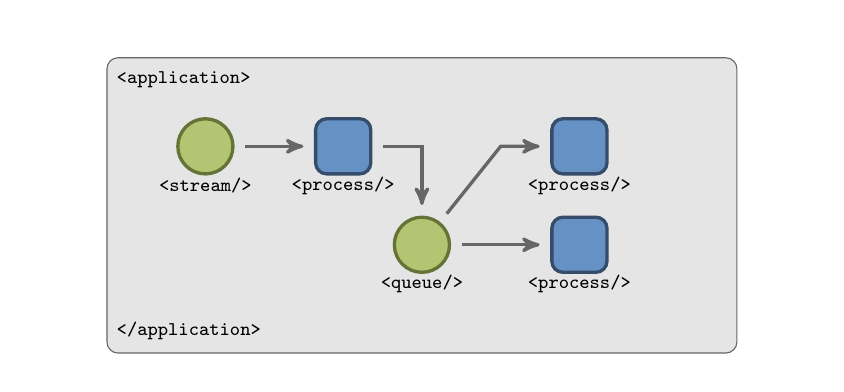
\begin{tikzpicture}
\node[rectangle, rounded corners, fill=black!10, draw=black!60, minimum width=8cm, minimum height=3.75cm] (A) at (0,0) {};
\node[anchor=west] at (-4,1.6) {\scriptsize{\ttfamily <application>}};
\node[anchor=west] at (-4,-1.6) {\scriptsize{\ttfamily </application>}};

\node[stream,scale=0.7] (S) at (-2.75,0.75) {};
\node at (-2.75,0.25) {\scriptsize{\ttfamily <stream/>}};

\node[process',scale=0.7] (P1) at (-1,0.75) {};
\node at (-1,0.25) {\scriptsize{\ttfamily <process/>}};

\node[stream,scale=0.7] (Q) at (0,-0.5) {};
\node at (0,-1) {\scriptsize{\ttfamily <queue/>}};

\node[process',scale=0.7] (P2) at (2,0.75) {};
\node at (2,0.25) {\scriptsize{\ttfamily <process/>}};

\node[process',scale=0.7] (P3) at (2,-0.5) {};
\node at (2,-1) {\scriptsize{\ttfamily <process/>}};

\draw[edge] (S) -- (P1);
\draw[edge,fill=none] (P1) -- (0,0.75) -- (Q);
\draw[edge,fill=none] (Q) -- (1,0.75) -- (P2);
\draw[edge] (Q) -- (P3);

\draw[draw=white] (-5,-2) rectangle (5,2.25);
\end{tikzpicture}

\caption{\label{fig:xml}The definition of a streaming application using XML elements.}
\end{figure}


Despite the specification of {\em process} elements of a data flow, the \textsf{streams}
framework allows for a more fine-grained control by defining each process by means of
a sequence of user-defined functions, called {\em processors}. These processors are
executed sequentially, each being applied to the data items, read by a process. Figure
\ref{fig:pipeline} shows the pipeline of user-defined functions (processors) for a process.
The profiling of these processor functions is the goal of the {\em streams-performance}
package.

\begin{figure}[h!]
\centering
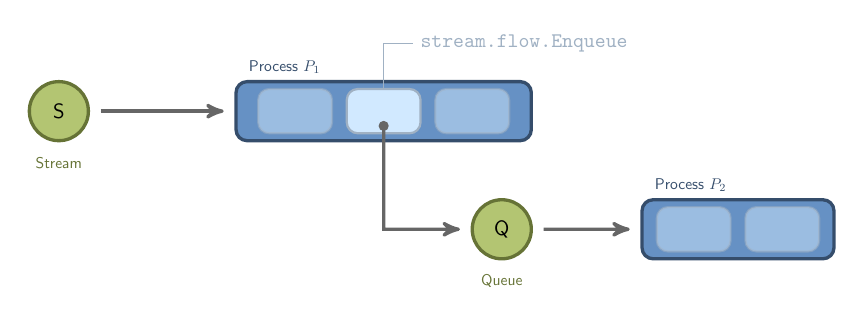
\begin{tikzpicture}[scale=0.75,transform shape]
\node[stream] (S) at (0,0) {
	\textsf{S}
};
\node[scale=0.75] at (0,-0.875){
	\color{gruenRand}\textsf{Stream}
};

\node[stream] (Q) at (7.5,-2) {
	\textsf{Q}
};
\node[scale=0.75] at (7.5,-2.875){
	\color{gruenRand}\textsf{Queue}
};

\node[anchor=west,scale=0.75] at (10,-1.25) {
	\color{blauRand}\textsf{Process $P_2$}
};
\node[process',minimum width=3.25cm] (P2) at (11.5,-2) {};
\node[processor,minimum width=1.25cm,opacity=0.5] at (10.75,-2) {};
\node[processor,minimum width=1.25cm,opacity=0.5] at (12.25,-2) {};

\node[anchor=west,scale=0.75] at (3.125,0.75) {
	\color{blauRand}\textsf{Process $P_1$}
};

\node[process',minimum width=5cm] (P1) at (5.5,0) {};
\node[processor,minimum width=1.25cm,opacity=0.5] at (4,0) {};
\node[processor,minimum width=1.25cm] (EN) at (5.5,0) {};
\node[processor,minimum width=1.25cm,opacity=0.5] at (7,0) {};

\draw[edge] (S) -- (P1);

\draw[hellblauRand] (EN.north) -- +(0,0.75) -- +(0.5,0.75);
\node[anchor=west] at (6,1.15) {
	\color{hellblauRand}{\ttfamily stream.flow.Enqueue}
};

\draw[edge,fill=none,shorten <=0pt] (5.5,-0.25) -- (5.5,-2) -- (Q);
\draw[fill=black!60,draw=black!60] (5.5,-0.25) circle (0.5ex);
\draw[edge] (Q)  -- (P2);
\end{tikzpicture}
\caption{\label{fig:pipeline}The execution pipeline of processors, defined within a process element.}
\end{figure}


\section{Profiling Processes}
The following objectives set the scene for the {\em streams-performance} package:
\begin{enumerate}
\item How much time does a specific processor require for each item?
\item What is the latency from reading an event to the time it is fully processed?
\item Which parts of the data item are read/written by each processor?
\end{enumerate}

The first two questions obviously aim at optimizing the individual processors. Improvements
here are generally code-based optimizations. With this aspect, the profiling provides an 
insight to easily identify the performance bottlenecks of a data flow graph. 
Figure \ref{fig:performancePlot} shows the accumulated processing times for a pipeline of
processors. The {\ttfamily CreateImage} processor is the element requiring the largest
amount of processing time.

\begin{figure}[h!]
\centering
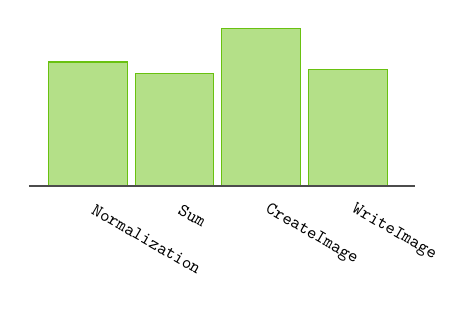
\begin{tikzpicture}
%
% path: 
\draw[color=blue,draw=gruen1,fill=gruen1!50](0.000,0.000) -- (1.000,0.000) -- (1.000,1.571) -- (0.000,1.571) -- (0.000,0.000);

\node[anchor=west,scale=0.65,rotate=-30] at (0.500,-0.250) {\ttfamily Normalization};
%
% path: 
\draw[color=blue,draw=gruen1,fill=gruen1!50](1.100,0.000) -- (2.100,0.000) -- (2.100,1.422) -- (1.100,1.422) -- (1.100,0.000);

\node[anchor=west,scale=0.65,rotate=-30] at (1.600,-0.250) {\ttfamily Sum};
%
% path: 
\draw[color=blue,draw=gruen1,fill=gruen1!50](2.200,0.000) -- (3.200,0.000) -- (3.200,2.000) -- (2.200,2.000) -- (2.200,0.000);

\node[anchor=west,scale=0.65,rotate=-30] at (2.700,-0.250) {\ttfamily CreateImage};
%
% path: 
\draw[color=blue,draw=gruen1,fill=gruen1!50](3.300,0.000) -- (4.300,0.000) -- (4.300,1.472) -- (3.300,1.472) -- (3.300,0.000);

\node[anchor=west,scale=0.65,rotate=-30] at (3.800,-0.250) {\ttfamily WriteImage};
%
% path: 
\draw[color=blue,draw=black!70,thick](-0.250,0.000) -- (4.650,0.000);

\end{tikzpicture}

\caption{\label{fig:performancePlot}Plot of the elapsed processing time for each processor.}
\end{figure}

Profiling the data access patterns of each processor can be seen as a more re-engineering
approach to determining which parts of the messages are relevant and might result in a
re-scheduling of the internal pipeline of the process executing the processors. For example,
if two processors compute and change disjoint properties of the messages, they might be
executing in parallel instead of a strict sequential execution.

Figure \ref{fig:access-graph} shows the access pattern of the same processing pipeline. As
can be seen in this figure, the {\ttfamily Sum} processor accesses the {\ttfamily data:normalized}
attribute and creates a new element {\ttfamily data:normalized:sum},
which in turn is not used by any of the succeeding functions. Thus, it would be safe to execute
the {\ttfamily CreateImage} and {\ttfamily WriteImage} functions in parallel to the {\ttfamily Sum}
processor.

\begin{figure}[h!]
\centering
\begin{tikzpicture}
\draw[white] (-6,0) rectangle (9,3);
\node[rotate=-30,anchor=west,scale=0.65] at (0.000,-0.750) {\ttfamily Normalization};
\draw[thin,draw=black!20] (-0.250,0.000) -- (0.000,0.000) -- (0.000,-0.500) ;
\node[circle,fill=gruen1,inner sep=0pt,minimum height=1.5ex,minimum width=1.5ex] at (-0.250,0.000) {};
\draw[thin,draw=black!20] (0.250,0.500) -- (0.000,0.500) -- (0.000,-0.500) ;
\node[circle,fill=orangeRand,inner sep=0pt,minimum height=1.5ex,minimum width=1.5ex] at (0.250,0.500) {};
\draw[thin,draw=black!20] (0.250,1.000) -- (0.000,1.000) -- (0.000,-0.500) ;
\node[circle,fill=orangeRand,inner sep=0pt,minimum height=1.5ex,minimum width=1.5ex] at (0.250,1.000) {};
\draw[thin,draw=black!20] (0.250,1.500) -- (0.000,1.500) -- (0.000,-0.500) ;
\node[circle,fill=orangeRand,inner sep=0pt,minimum height=1.5ex,minimum width=1.5ex] at (0.250,1.500) {};
\node[rotate=-30,anchor=west,scale=0.65] at (1.000,-0.750) {\ttfamily Sum};
\draw[thin,draw=black!20] (0.750,1.500) -- (1.000,1.500) -- (1.000,-0.500) ;
\node[circle,fill=gruen1!60,inner sep=0pt,minimum height=1.5ex,minimum width=1.5ex] at (0.750,1.500) {};
\draw[thin,draw=black!20] (1.250,2.000) -- (1.000,2.000) -- (1.000,-0.500) ;
\node[circle,fill=orangeRand,inner sep=0pt,minimum height=1.5ex,minimum width=1.5ex] at (1.250,2.000) {};
\node[rotate=-30,anchor=west,scale=0.65] at (2.000,-0.750) {\ttfamily CreateImage};
\draw[thin,draw=black!20] (1.750,2.500) -- (2.000,2.500) -- (2.000,-0.500) ;
\node[circle,fill=gruen1,inner sep=0pt,minimum height=1.5ex,minimum width=1.5ex] at (1.750,2.500) {};
\draw[thin,draw=black!20] (1.750,1.500) -- (2.000,1.500) -- (2.000,-0.500) ;
\node[circle,fill=gruen1!60,inner sep=0pt,minimum height=1.5ex,minimum width=1.5ex] at (1.750,1.500) {};
\draw[thin,draw=black!20] (2.250,3.000) -- (2.000,3.000) -- (2.000,-0.500) ;
\node[circle,fill=orangeRand,inner sep=0pt,minimum height=1.5ex,minimum width=1.5ex] at (2.250,3.000) {};
\node[rotate=-30,anchor=west,scale=0.65] at (3.000,-0.750) {\ttfamily WriteImage};
\draw[thin,draw=black!20] (2.750,3.000) -- (3.000,3.000) -- (3.000,-0.500) ;
\node[circle,fill=gruen1!60,inner sep=0pt,minimum height=1.5ex,minimum width=1.5ex] at (2.750,3.000) {};
\node[scale=1.0,anchor=east,scale=0.5] at (-1.000,0.000) {\color{black!80}{\ttfamily data:raw}};
\node[scale=1.0,anchor=east,scale=0.5] at (-1.000,0.500) {\color{black!80}{\ttfamily data:min}};
\node[scale=1.0,anchor=east,scale=0.5] at (-1.000,1.000) {\color{black!80}{\ttfamily data:max}};
\node[scale=1.0,anchor=east,scale=0.5] at (-1.000,1.500) {\color{black!80}{\ttfamily data:normalized}};
\node[scale=1.0,anchor=east,scale=0.5] at (-1.000,2.000) {\color{black!80}{\ttfamily data:normalized:sum}};
\node[scale=1.0,anchor=east,scale=0.5] at (-1.000,2.500) {\color{black!80}{\ttfamily data:samples}};
\node[scale=1.0,anchor=east,scale=0.5] at (-1.000,3.000) {\color{black!80}{\ttfamily image:png}};
\begin{scope}[scale=0.75,transform shape,shift={(2.5,-1)}]
\node[circle,fill=orangeRand,inner sep=0pt,minimum height=1.5ex,minimum width=1.5ex] at (5,0) {};
\node[anchor=west,scale=0.75] at (5.25,0) {\ttfamily write access};
\node[circle,fill=gruen1,inner sep=0pt,minimum height=1.5ex,minimum width=1.5ex] at (5,-0.5) {};
\node[anchor=west,scale=0.75] at (5.25,-0.5) {\ttfamily read access};
\node[circle,fill=gruen1!50,inner sep=0pt,minimum height=1.5ex,minimum width=1.5ex] at (5,-1) {};
\node[anchor=west,scale=0.75] at (5.25,-1) {\ttfamily read access to written field};
\end{scope}

\end{tikzpicture}
\caption{\label{fig:access-graph}Access graph of a processing pipeline of four processors.}
\end{figure}


\section{Profiling streams Applications}
The profiler of the {\em streams-performance} package is a drop-in implementation for replacing
the default {\em process} implementation of \textsf{streams}. By using the {\ttfamily class}
attribute of the process element, the implementation {\ttfamily streams.profiler.Process} can
be used to monitor processor performances and data accesses. The resulting profile will be
written to an XML file, which holds the process configuration, enriched by performance numbers
and field access information.

Figure \ref{fig:profilerExample} show the process specification for profiling a simple processor
pipeline using the {\em streams-performance} package. The {\ttfamily file} attribute is used to
define the output file for the profiling information.

\begin{figure}[h!]
\centering
\begin{tikzpicture}
\node at (0,0) {
\begin{lstlisting}[language=XML]
        <process input="data" class="streams.profiler.Process"
                  file="/profiling.xml">
           <example.Normalization />
           <example.Sum />
           <example.CreateImage />
           <example.WriteImage />
        </process>
\end{lstlisting}
};
\draw[thick,orangeRand] (-0.3,1.05) rectangle (5.85,1.5);
\draw[thick,orangeRand] (5,1.05) -- (5,0.5);
\node[scale=0.65] at (5,0.2) {\textsf{Profiler Process Implementation}};
\end{tikzpicture}
\caption{\label{fig:profilerExample}Replacing the default process implementation to gain profiling information.}
\end{figure}

As mentioned before, the profiling data is written to an XML file. The package provides Java classes
to parse and plot these files. The output is written as TeX files using the {\em tikz} package. To
produce a performance plot from XML produced by the profiler, you need to run:
\begin{center}
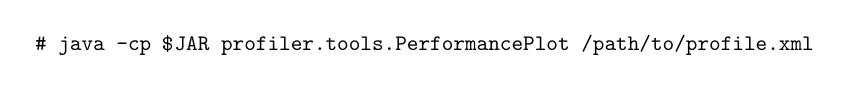
\begin{tikzpicture}
  \node[scale=0.8,anchor=west] at (0,0) {\ttfamily \# java -cp \$JAR profiler.tools.PerformancePlot /path/to/profile.xml};
\end{tikzpicture}
\end{center}
where {\ttfamily \$JAR} denotes the {\em streams-performance} Java archive file.

With the {\ttfamily profiler.tools.AccessGraph} class, the data access graph can be plotted from the
same XML data file:
\begin{center}
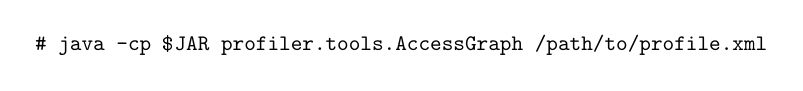
\begin{tikzpicture}
  \node[scale=0.8,anchor=west] at (0,0) {\ttfamily \# java -cp \$JAR profiler.tools.AccessGraph /path/to/profile.xml};
\end{tikzpicture}
\end{center}

\end{document}